\documentclass[doctor, openright, oneside]{gdutthesis}
\usepackage{zhlipsum}

\begin{document}

\frontmatter % 正文前的摘要部分(罗马数字页码)

% 生成封面
\maketitle

% 生成书脊
% \spine

%%%%%%%%%%
% 摘要
%%%%%%%%%%

\begin{abstract}{chinese}
反射式光纤位移传感器由于具有原理简单、实现容易、工作可靠等诸多优点而受到
越来越广泛的重视。本系统由于要同时兼顾高精度和大量程的要求,因此在反射式光纤
位移传感器的一般原理上进行了新的设计,使它较好的达到了实际的设计要求。鉴于本
项目中光纤传感头的设计与实现工作已经基本完成,本文主要侧重于对电路部分的设计
与调试工作进行描述。\par
......\par
\end{abstract}

\begin{abstract}{english,continue=true}
Fiber-optic reflective displacement sensor attracts much attention for its particular
advantages, such as simply theory, easy realization, good stability and so on. With the
requirement of wide measurement range and high precision, it is re-designed based on the
basic principle of the simplest reflective fiber-optic sensor. For some work having been
finished at the beginning of this project, I will mainly describe the electric circuit.\par
......\par
\end{abstract}

% 生成目录
\tableofcontents

\mainmatter % 正文开始(阿拉伯数字页码)

% 诸论
\chapter{诸论}
\section{本题目的目的及意义}
\section{研究范围及要达到的技术要求}
\section{国内外的发展概况及存在的问题}
\section{本题目的指导思想及应解决的主要问题}



% 正文
%\chapter{正文主体}
\section{问题的提出}
\section{研究工作的基本前提以及假设和条件}
\section{模型的建立以及实验方案的拟定}
\section{基本概念和理论基础}
\section{设计计算的主要方法和内容}
\section{实验方法实验内容及其分析}
\section{理论论证}
\section{理论在题目中的应用}
\section{题目得出的结果}
\section{对结果的讨论}

%\input{tex/chapter2} % 可以按章分开各个文件
%...

\chapter{I 级叶/盘协调转子固有振动特性分析}
\section{基础知识}
\subsection{有限元法}
\subsection{循环对称结构的分析方法}
\section{I 级叶/盘转子振动特性的有限元分析}
\subsection{计算模型}

\subsection{有限元计算结果及分析}

\chapter{I级叶/盘转子错频方案的对比分析}

在叶轮机械领域,对一个实际的叶盘转子,错频是指由于单个叶片之间因几何上
或结构上的不同而造成的其在固有频率上的差异。\par

......\par

\section{多自由度系统的强迫响应分析}

由前面的分析可知,响应分析在数学上是一个具有 38 个自由度的二阶线性微分方
程的数值积分问题。\par

\subsection{动态响应的计算方法}

\begin{enumerate}
\item 系统的运动方程\\
多自由度系统运动微分方程的一般形式为:
\begin{enumerate}
\item $\cdots$
\item $\cdots$
\end{enumerate}
\item 微分方程组的数值积分\\
一阶常系数微分方程组的初值问题可表述为: ......
\end{enumerate}

\subsection{强迫响应分析前的准备工作}
......\par

\chapter{\LaTeX 示例}
\section{公式}
\begin{equation}
\vec{P}_{i}(u)=\sum_{j=0}^{k} \vec{V}_{i} \Lambda_{i}\left(k ; \vec{\beta}_{1}, \cdots \vec{\beta}_{n} ; u\right)
\end{equation}

\begin{equation}
\frac{|A(s)|^{2}}{|A(o)|^{2}}=\frac{\rho_{1} \rho_{2}}{\left(s+\rho_{1}\right)\left(s+\rho_{2}\right)}
\end{equation}

\section{表格}

\begin{table}[h]
\centering
\caption{压降损失计算结果}
\label{table:jiangya}
\begin{tabularx}{\textwidth}{CCC}
\toprule[2pt]
换热器&热边压降损失&冷边压降损失\\
\midrule[1pt]
初级&2974.37&2931.52\\
次级&2924.65&3789.76\\
\bottomrule[2pt]
\end{tabularx}
\end{table}

\section{图}


\begin{figure}[!h]
\centering
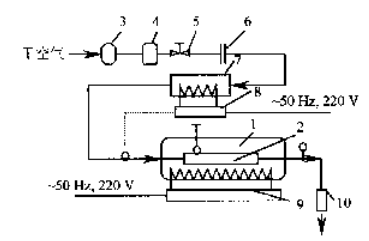
\includegraphics[width=0.5\textwidth]{figures/danguan}\\
\footnotesize
1-太阳模拟器;2-单管及 31 个 PCM 容器;3-气泵;\\
4-干燥过滤器;5-手动调节阀;6-孔板流量计;\\
7-空气预热器;8,9-调功器;10-空气换热器.\\
\caption{单管换热系统流程图}
\label{fig:danguan}
\end{figure}


\begin{figure}[!h]
  \subfigure[t][分布符合 $1 / f$ 规律图]{
    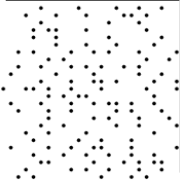
\includegraphics[width=0.25\textwidth]{figures/a}
  }
  \hfill
  \subfigure[t][大小与色彩符合 $1 / f$ 规律图]{
    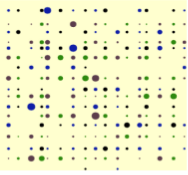
\includegraphics[width=0.25\textwidth]{figures/b}
  }
  \hfill
  \subfigure[t][间距、大小与色彩均符合 $1 / f$ 规律图]{
    
\includegraphics[width=0.25\textwidth]{figures/c}
  }
  \caption{图案例}
  \label{fig:tuan}
\end{figure}


% 结论
\chapter{结论}
\section{对所得结果与已有结果的比较}
\section{题目尚存在的问题}
\section{进一步开展研究的见解与建议}


% 参考文献
\printbibliography[heading=bibintoc]

\begin{appendix}
\appendixpage% 插入“附录”字样的分割页

\chapter{附录1标题}
\section{附录1节标题}

\chapter{附录2标题}

\end{appendix}


\backmatter % 文后无编号部分

% 致谢
\begin{thanks}
\zhlipsum % 生成假文
\end{thanks}


\end{document}
